\chapter{Edges}
\label{sec:edges_background}
\begin{figure}
    \centering
    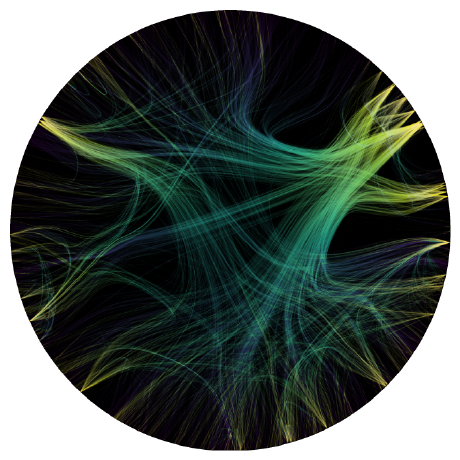
\includegraphics[width=.6\textwidth]{power/figures/metaunityplaceholder.png}
    \caption{A visualisation of the Unity game engine, produced using the Unity game engine. TODO: explanation of hierarchy and labels around perimeter. Also move this to the start of the chapter}
    \label{fig:metaunity}
\end{figure}
The previous chapter of was an exploration of how to position the vertices of a graph, and the natural question to then ask is how to deal with the only remaining component: the edges. However this question is seemingly redundant at first, as the obvious answer is to simply draw straight lines between adjacent nodes. While this by no means a poor choice, and is exactly how all node-link diagrams have been drawn thus far, this chapter will explore the possibility of drawing links using curves instead.

\section{Background}
The curving of links in the context of a node-link diagram is known as \textit{edge bundling}. It is a technique that has been developed because many networks, when processed through a standard force-directed layout, result in a seemingly random layout with no discernable structure. See Figure~\ref{TODO} for an example. The similarity of such layouts to tangled piles of hair has led to them being colloquially termed \textit{hairballs}.

Unfortunately this is not an easily solved problem, because the \textit{curse of dimensionality} \cite{Friedman2001} means that most of these networks simply cannot be accurately represented in two dimensions, and the likelihood of this problem only rises as the size of any network increases. This is all even if there is a clear underlying structure to these networks, lying beyond the reach of the standard layout algorithm.
Edge bundling attempts to alleviate this issue by introducing a trade-off---the ability to follow individual links is sacrificed for better representation of global structure, by allowing links to overlap.

This is analogous to organising the wires in a computer system by tying groups of wires together that share similar endpoints. A simple example of this is illustrated in Figure~\ref{TODO}, where the compromise between being able to follow links showing global structure is clearly visible.

The literature is rich with various different methods for performing this bundling, dating all the way back to the 1800s with the flow maps of Minard \cite{Minard1862} or Sankey diagrams \cite{Sankey1896}.
More modern algorithms for performing bundling automatically include multilevel agglomerative edge bundling (MINGLE) by Gansner et al.~\cite{Gansner2011} which greedily merges pairs of links at a time by selecting the pairs that minimise a cost function based on the amount of `ink' used to draw links. A more complex cost function is used in metro-style bundling by Pupyrev et al.~\cite{Pupyrev2016}, which is based on multiple criteria including ink, individual edge lengths and node separations. 
The same premise behind force-directed node layout is also used in force-directed edge bundling by Holten and van Wijk \cite{Holten2009}, which bundles links by defining forces between adjacent links instead of nodes. As shown previously in Section~\ref{sec:force_background}, force-based methods are in fact gradient descent optimisation methods where the gradient is defined before the cost function itself, and this edge bundling technique is no different.

Another effective approach is \emph{kernel density estimation} by Hurter et al.~\cite{Hurter2012}, who iteratively apply a convolutional filter over a density map of links in an already rendered diagram. This method belongs to the subfield of image-based bundling methods \cite{Lhuillier2017,Telea2018}. A diverse gallery of edge bundling algorithms applied to the same dataset can be see in the review of Lhuilier et al.~\cite[Fig.~4]{Lhuillier2017}.
However all of the aforementioned methods share a key similarity: they apply bundling upon the assumption that node positions are predetermined and will not be moved. This is perfectly fine and even desirable in many common use cases where nodes have a predefined location, such as geographical maps, but methods such as force-directed layouts were never designed to place similar edges in parallel. In fact, the angular resolution of edges sharing nodes is sometimes used as part of the optimised cost function \cite{Argyriou2010}) and so common layout methods usually do not help, if not worsen, the bundling quality of their visualisations.

This is why one of the most powerful network visualisation techniques is method known as \emph{hierarchical edge bundling}, published by Holten in 2006 \cite{Holten2006}\footnote{Its effectiveness was recognised by a `Test of Time' award at the IEEE VIS conference in 2016.}
An example of this in action can be seen in Figure~\ref{fig:metaunity}, which contains the method applied to the source code of the Unity game engine. The graph being visualised is a call graph, where each class is a vertex, and is connected by an edge to any other class it depends on. 

The trick to the bundling comes from the fact that we have extra metadata available: the hierarchy of folders and source files that holds the code.
This hierarchy, not the call graph itself, is first layed out as a tree. Then, since this tree includes extra nodes to represent the folders and source files, these extra nodes are erased from the final visualisation. However their coordinates are instead used as an auxiliary routing graph (ARG) through which the call graph edges are routed through.
More precisely, this process of routing involves taking every edge in the call graph, and rendering each one using a spline curve whose control points consist of a path through the ARG. The precise definition of this spline is important, and will be further elaborated upon in Section~\ref{TODO}, but for now the important thing to note is that this produces bundling behaviour because vertices close to each other in the hierarchy will share control points for their splines, thus curving their rendered links towards each other.
The hierarchical tree extracted from the Unity game engine can be seen on the TODO hand side, to illustrate its influence on the final visualisation. 

This technique is so effective because the structure of the bundles is informed by human judgement. To continue within the call graph example, the hierarchy of folders and source files is literally designed by the programmers for organisational purposes, and so it is very likely to admit some utility for also organising, say, a visualisation.
Additionally, not only is the curvature links influenced by the ARG, but so is the position of the nodes. Since each node is a leaf in the tree-shaped ARG, their positions around the circle are also influenced by the topology of the tree, which on its own already vastly improves the quality of the layout.
This idea of using an auxiliary hierarchy to inform bundling is the basis of the work in this chapter, except that I will instead investigate the more common situation of when this metadata is not included with the original data. It must therefore must be generated by the algorithm itself as a preprocessing step.

\subsection{Clustering}
What is needed is a way of grouping similar datapoints together. This is known as \textit{clustering}, and is a vast field of study, not least as one of the primary objectives of the fast-growing discipline of machine learning. The subfield of clustering just within the context of networks is large in its own right, due to its utility in common datasets such as protein--protein interaction or social networks.

There exist a wide variety of powerful and creative methods that have been developed to perform clustering on networks. A widely used method is to define an equation that can be used to numerically measure the quality of a given clustering, and to attempt to maximise this quality. This is reminiscent of the optimisation-based methods described in Section~\ref{sec:force_background}.
A popular version of this is known as \emph{modularity}, defined as
\begin{equation}
Q = \frac{1}{|E|}\sum_{i,j}\left(\mathbf{A}_{ij} - \frac{|N(i)||N(j)|}{|E|}\right)\mathbf{C}_{ij}
\label{eq:modularity}
\end{equation}
where $\mathbf{A}$ is the adjacency matrix where $\mathbf{A}_{ij}$ equals 1 if vertices $i$ and $j$ are connected by an edge, and $\mathbf{C}_{ij}$ equals 1 if vertices $i$ and $j$ are in the same cluster and 0 otherwise.
The value of $Q$ lies between $-\frac{1}{2}$ and 1 \cite{Brandes2007a}, and it can be intuitively understood as the fraction of the edges that fall within the given clusters minus the expected fraction if edges were distributed at random.

This was introduced by Newman and Girvan \cite{Newman2004} to evaluate a separate clustering algorithm, and later directly optimised by Newman \cite{Newman2006} with two methods that both initialise the network as one big cluster that is recursively split into half until no further gain in modularity is possible. The first finds the split by calculating eigenvectors of the \emph{modularity matrix}, and another that finds the split by repeatedly moving vertices between the two sides of the split until modularity is maximised, akin to a hill-climbing method.
Optimising modularity in general is $\mathcal{NP}$-complete \cite{Brandes2007a}, but its intuitive interpretation has led to various other authors to develop methods to optimise it. The Louvain algorithm (given its name from the authors coming from the University of Louvain, Belgium) \cite{Blondel2008} and its recent improvement to the Leiden algorithm (from Leiden University, Netherlands) \cite{Traag2019} both start by placing every vertex in a singleton cluster and successively merging clusters whilst also moving vertices between clusters, also until modularity cannot be improved further.

The behaviour of random walks along the graph has also been used to great effect for clustering. For example, the \emph{markov cluster} algorithm of Enright et al.~\cite{Enright2002} simulates a random walk process through a series of matrix multiplications on the markov chain of the graph.
The \emph{infomap} algorithm of Rosvall and Bergstrom \cite{Rosvall2008} optimises a cost function known as the map equation, which applies information-theoretic concepts such as entropy to the behaviour of random walkers. It is optimised through a combination of greedy search and simulated annealing.
Other types of algorithms include statistical inference methods such as Bayesian inference \cite{Hastings2006} and block-modelling \cite{Reichardt2007}.
Another perspective on clustering includes grouping together edges instead of vertices, which means that a single vertex may belong to many overlapping clusters, an idea explored by Evans and Lambiotte \cite{Evans2009}.
The growing number of graph-shaped datasets being used in machine learning has also led to a number of supervised and semi-supervised methods for clustering and general dimensionality reduction, such as \emph{DeepWalk} \cite{Perozzi2014} which treats each vertex as a `word' to generate `sentences' using random walks across vertices. These sentences are then taken and applied to techniques originally designed for language processing. Attempts to transfer the success of convolutional neural networks have also been generalised to apply to graphs of any topology \cite{Kipf2016, LeCun2017}, as well as many other architectures depending on the task at hand \cite{Battaglia2018, Wu2020}.

% The variety of different methods available is in part due to one key characteristic of network clustering: it is an undefined problem.
One reason why there is such a variety of clustering algorithms is due in part to it being an undefined problem.
Clustering can be likened to data compression, as the goal is to describe a given network with less information than, say, viewing the source and target of every individual edge. Such compression would be impossible in a random network, but because real-world data does have structure, underlying patterns can be leveraged to group together similar components within the data.
However, even knowing that this is the goal does not make the problem easier, because these underlying patterns are not known to us. The real world is complex, and so any data collected from it is not likely to be straightforward to understand. Much of the data collected may not even contain any order in the first place.
% In fact, if you will allow me to go meta for a moment, the very act of collecting data itself into the form of a network is already technically a form of compression, as 
It is therefore important to keep in mind that clustering algorithms are attempts to quantify common characteristics of real-world data, and there is generally no `right answer' to the question of which one should be chosen.
It depends on both the specific objective and dataset being examined. Nevertheless, they have been used to great effect in many applications \cite{Fortunato2016}, and so confidence can be placed in their utility as a tool to help understand patterns in data.

The work in this chapter will focus on \emph{hierarchical clustering}, the family of clustering algorithms where the output is a \textit{dendrogram}: a binary tree used to describe a hierarchical structure.
This can either be done from the bottom up, i.e.\ each node starts in its own cluster and pairs of clusters are progressively merged until only one remains, or top down, i.e\ every node starts in the same cluster that is recursively split into two halves. The former is known as \emph{agglomerative} clustering, and the latter as \emph{divisive} clustering.
The output fits well with our purposes, since our goal is to construct a hierarchical edge bundling visualisation like the one in Figure~\ref{fig:metaunity}, but without a prior hierarchy included with the data; the dendrogram produced from such a clustering algorithm can be used as this missing hierarchy.

This idea of using the output dendrogram of a clustering algorithm to produce hierarchical edge bundling has been previously explored by Jia et al.~\cite{Jia2011}\footnote{TODO: bad splines}, who produce a hierarchy using the algorithm of Newman and Girvan \cite{Newman2004}, known commonly as the Girvan-Newman algorithm. This method removes one edge from the network at a time, specifically the one with the most \emph{betweenness centrality} i.e.\ the edge traversed the most often when mapping the shortest paths between all pairs of vertices. This naturally splits clusters when an edge is removed that is the final bridge between two clusters.
Unfortunately Jia et al.\ did not perform any quantitative analysis to evaluate the performance of their clustering algorithm, and only present results when using one clustering method. The work in the following section will aim to extend their work by evaluating the performance of a number of hierarchical clustering methods, against a benchmark of graphs where the ground truth cluster configuration is known.

\section{Hierarchical Clustering}
\begin{figure}
    \centering
    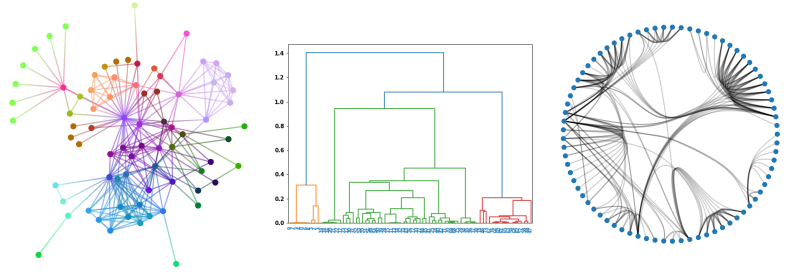
\includegraphics[width=\linewidth]{power/figures/lesmis.png}
    \caption{An example of the target: edges have weights, todo: move circle to bottom with plus sign}
    \label{fig:lesmis}
\end{figure}
To assess the quality of the divisive Girvan-Newman algorithm used by Jia et al.~\cite{Jia2011}, it will be compared with \emph{agglomerative dissimilarity clustering}.
This is a family of algorithms where the input is a matrix of \emph{dissimilarities} between individual datapoints, in this case the vertices of a graph, and the output is a dendrogram as required. Similarly to the stress-based layout explored in the previous chapter, it is a more general algorithm that can be applied to any numerical datasets and not just graphs, unlike the methods previously outlined in Section~\ref{sec:edges_background}. It is also closely related to the class of multidimensional scaling methods that stress minimisation belongs to, as both procedures take a matrix of dissimilarities as input.

Not only does this fit thematically with the topics explored in previous chapters, but a key benefit to using dissimilarity clustering is that the output dendrogram contains extra information to describe the `quality' of the merge at that point. This information is vital as it can be used to `prune' the hierarchical tree in order to make the resulting edge bundles more salient. This will be elaborated upon in Section~\ref{sec:pruning}.
Two other questions must first be answered before we can proceed with performing this clustering: what exactly are the dissimilarities to be used as our input, and how will the algorithm proceed to process these dissimilarities to merge clusters? These will both be answered in the following section.

\subsection{Dissimiliarity Clustering}
\label{sec:dissimilarities}
General hierarchical clustering based on dissimilarities can be done in both an agglomerative and divisive way, but the work here will focus on agglomerative methods. Agglomerative methods are more popular among practitioners \cite{Roux2018} due largely to the divisive version having $\mathcal{O}(2^n)$ possible splits for a cluster of size $n$, as each datapoint can be placed in either one half or the other. This results in an exponential runtime complexity per split, whereas the agglomerative method has only to chose from pairs of datapoints per merge, giving an $\mathcal{O}(n^2)$ complexity.

There do exist heuristics to speed up the divisive method to bring the complexity down to polynomial, such as using algorithms like k-means to decide the split instead \cite{Lamrous2006}.
% It can also be argued that a divisive method can take a more global approach.
However, since we already have a graph-specific divisive method in the Girvan-Newman algorithm to compare to, the work on this chapter will focus on comparing it to its agglomerative counterparts.

\subsubsection{Greedy Agglomeration}
The agglomerative process is as follows:
% \begin{tabular}
% \cellcolor{green!15}{
% }
% \end{tabular}

\begin{mdframed}[backgroundcolor=WhiteSmoke]
\begin{enumerate}[leftmargin=*]
    \item Calculate the distances between all pairs of datapoints. \label{item:agglomerate_calculate}
    \item Place each datapoint into its own singleton cluster.
    \item Iterate over each pair of clusters, and merge the closest pair into a single cluster. \label{item:agglomerate_pairs}
    \item Recalculate the distances between the newly merged cluster and the remaining unmerged clusters. \label{item:agglomerate_recalculate}
    \item Repeat steps \ref{item:agglomerate_pairs} and \ref{item:agglomerate_recalculate} until only one supercluster remains.
\end{enumerate}
\end{mdframed}
On the surface this is a simple procedure, but it is not immediately clear how to calculate distances between datapoints or between clusters in steps \ref{item:agglomerate_calculate} or \ref{item:agglomerate_recalculate}.
There are an abundance of choices for what to use for step \ref{item:agglomerate_calculate}, which is the same first step as used in stress-minimisation from Section~\ref{sec:stress_background}. There, the graph-theoretic shortest-path was used as the dissimilarity, but it will soon be made clear that this is far from an optimal choice. An experimental comparison between I will start by assuming that we have a dissimilarity already defined between graph vertices, and first discuss how to recalculate

Unweighted is, perhaps confusingly, more precise than the weighted version (directly opposite to the case in weighted and unweighted shortest paths). 
UPGMA WPGMA
ward is simply better because of things, and so it is the only type we will test here
% Another benefit to agglomerative methods is that it is easy to interpret and understand what the algorithm is doing, even if the answer is suboptimal. I would always pick an algorithm that I fully understand for a visualisation over a black-box algorithm that produces slightly better results. But this is just opinion.

describe lance-williams to derive complexity!

Shortest paths were used in the previous chapter, but they don't work here because...
We therefore use the variation - multiply by jaccard distance
note that Ward strictly requires a distance metric


\subsubsection{Random Walks as Dissimilarities}
The first step is to embed in high dimensional space.
an extra benefit is that we can use edge weights (unlike other algorithms, see Figure~\ref{fig:lesmis}
say laplacian is kirchoff for commute distance

damped or snapshot
 - I expect damped to be more smooth
 - I also expect both to converge to the same result (damp=1 vs steps=inf

note that walktrap only merges along edges, so it does not require the $n^2$ calculation every time

best answer is walktrap 5, and original authors seemed to agree...

\subsection{Experimental Study}
\label{sec:clustering_experiment}
since clustering is actually an undefined problem. So I will test against ground truth data
describe datasets that have ground truths along with citations
\begin{itemize}
    \item karate
    \item football
    \item caltech
    \item lfr
\end{itemize}
describe ARI
\begin{itemize}
    \item divisive girvan-newman -- this results in long strands that suck
    \item embedding methods: walktrap + KL + wasserstein
    \item jaccardsp, commute
    \item also tested louvain and infomap, although they do not generally produce a dendrogram
\end{itemize}
\begin{figure}
    \caption{TODO: big grid of ARI}
    \label{fig:ARI}
\end{figure}

\subsection{Pruning}
\label{sec:pruning}
\begin{figure}
    \caption{Caption}
    \label{fig:pruning}
\end{figure}
However the problem with using a dendrogram is that, as a binary tree, it contains as many branch nodes as leaves, which means that the resulting splines have far too many control points to be meaningful. An example of this can be seen in Figure~\ref{fig:lesmis}.
Jia et al.~\cite{Jia2011} attempt to alleviate this by introducing 
but GN complexity is also ridiculous

mention the optimal ordering from Scipy, Bar-Joseph et al.~\cite{Bar-Joseph2001}, around a circle

merge branches in tree to make pretty
optimal leaf ordering also pretty
Garland paper does pruning of top down
mention that pruning is not the only way to do things e.g. skipping more control points. YMMV

END THIS CHAPTER WITH PSEUDOCODE

\subsection{Discussion}
but this is all kind of besides the point for HEB because the kind of structure we want to reveal is not clique structure, but biclique structure.
% it is very important to realise that there are two types of clusters, which will be henceforth referred to as 'community' and 'betweenness' structure. This can also be referred to as 'assortative' and 'disassortative'.
% some networks have both at the same time, and it is therefore difficult

\section{Power-confluent Drawings}
\begin{figure}
    \caption{TODO: teaser image in pconfluent paper}
    \label{fig:power_teaser}
\end{figure}
in confluent drawings the aforementioned trade-off is actually attempted to be avoided
it is likened to lossless compression.

2 parts: finding the power groups, then converting to a confluent drawing. The results here improve the speed and quality of the first part, and fix theoretical issues with the second.
The nested structure of power-groups is hierarchical, and so an agglomerative method is used.
\subsection{Splines}
b-spline algorithms and things
holten qualitatively said some desirable properties of b-splines, but the real benefit of them is the convex hull property, which helps to prevent crossings (explain why... because)
The importance of this has been crucially missing in the literature
examples of splines that are not convex hull is like the garland paper.
